\documentclass[notitlepage, 12pt]{article}

\usepackage{amssymb}           % dodatni simboli
\usepackage{amsmath}           % eqref, npr.
\usepackage[pdftex]{graphicx}
\usepackage{amsthm}
\usepackage{tikz}
\usepackage[dvipsnames]{xcolor}
\usepackage{svg}

\usepackage{geometry}
\geometry{
  a4paper,
  total={160mm,257mm}, % total width and height of the text
  left=25mm, % left margin
  right=25mm, % right margin
}



\graphicspath{ {./img/} }

\title{Teorija grafov - Zapiski predavanj}
\author{Jakob Drusany}

\newtheorem*{definition}{Definition}
\newtheorem*{theorem}{Theorem}
\newtheorem*{lemma}{Lemma}
\newtheorem*{example}{Example}

\begin{document}
\maketitle
\vspace{1cm}
\tableofcontents
\thispagestyle{empty}
\newpage
\pagenumbering{arabic} 
\section{Introduction}
A graph is defined as $G = (V, E)$. $n = |V|$ is the number of vertices, $m = |E|$ is the number of edges.
We also denote them as $V(G), n(G)$, $E(G), m(G)$. $\delta(G)$ is the minimum degree of a vertex in $G$, $\Delta(G)$ is the maximum degree.
$G[C]$ represents the induced subgraph of $G$ on the vertex set $C$.
\section{Independence, matching, covers}
\begin{definition}
  The set of vertices $S \subseteq V$ is an \textbf{independent set} if $G(S)$ contains no edges.
  (No two vertices in the independent set are adjacent)
\end{definition}
The independence number $\alpha(G)$ is the size of the maximum independent set.
\begin{definition}
The set of vertices $T \subseteq V$ is a \textbf{vertex cover} if $\forall e \in E$ $T \cap e \neq \emptyset$.
(All edges have at least one endpoint in the vertex cover)
\end{definition}
The vertex cover number $\beta(G)$ is the size of the minimum vertex cover.
\begin{definition}
  A \textbf{matching} is a set of edges $M \subseteq E$ such that $\forall e, f \in M$ $e\neq f$ $e\cap f\neq \emptyset$.
  (No two edges share a vertex)
\end{definition}
The matching number $\alpha'(G)$ is the size of the maximum matching.
\begin{definition}
  An \textbf{edge cover} is a set of edges $C \subseteq E$ such that $\forall v \in V$ $\exists e \in C$ $v \in e$.
  (All vertices are covered by at least one edge from $C$)
\end{definition}
The edge cover number $\beta'(G)$ is the size of the minimum edge cover.
Some graphs have no edge covers, for example graphs with isolated vertices.

\begin{example}
    \begin{figure}[h]
      \includegraphics[width=0.8\textwidth]{first_example.pdf}
      \centering
      \caption{$G$ from example}
    \end{figure}

    % text colored red
    \textcolor{BrickRed}{$\alpha(G) = 8$}\\
    \textcolor{blue}{$h(G) = 20$}\\
    \textcolor{OliveGreen}{$\beta(G) = 12$} $\rightarrow$ complement of vertex set\\
    \textcolor{Dandelion}{$\alpha'(G) = 10$} maximum for $\alpha'$ is $\frac{h(G)}{2}$\\
    \textcolor{purple}{$\beta'(G) = 10$}
\end{example}
\newpage
\Large{Observations} \normalsize
\begin{itemize}
  \item $\alpha(G) + \beta(G) = |V|$ (the size of the maximum independent set plus the size of the minimum vertex cover is equal to the number of vertices)
  \begin{proof}
    For every independent set $S$, the complement $\overline{S}$ is a vertex cover and vice versa.
  \end{proof}
  $\alpha'(G) \leq \beta(G)$ (the size of the maximum matching is less than or equal to the size of the minimum vertex cover)
  \begin{figure}[h]
    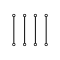
\includegraphics[width=0.2\textwidth]{matching-number-smaller-than-vertex-cover.pdf}
    \centering
  \end{figure}
  \begin{proof}
    Every edge in a maximum matching must be covered by different vertices in the vertex cover.
  \end{proof}
  \item $\alpha(G) \leq \beta'(G)$ (the size of the maximum independent set is less than or equal to the size of the minimum edge cover)
  \begin{proof}
    Every vertex in a maximum independent set must be covered by different edges in the edge cover.
  \end{proof}
  \item if $G$ has no isolated vertices: $\alpha'(G) \leq \frac{n}{2} \leq \beta(G)$
  \begin{figure}[h]
    
\includegraphics[width=0.2\textwidth]{matching-number-smaller-than-vertex-cover-2.pdf}
    \centering
  \end{figure}
\end{itemize}
\newpage
\begin{theorem}[Galloi's theorem]\label{gallois-theorem}
  If $G$ has no isolated vertices, then $\alpha'(G) + \beta'(G) = n(G)$.
\end{theorem}
\begin{proof}
\begin{itemize}
    \item[(1)] $\beta'(G) + \alpha'(G) \leq |V(G)|$ \\ \newline
    \begin{figure}[h]
      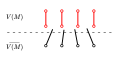
\includegraphics[width=0.4\textwidth]{gallois-theorem-1.pdf}
      \centering
    \end{figure}
    Take a maximum matching $M$; $M = \alpha'(G)$. For every vertex not covered
    in $M$ ($\overline{V(M)}$), we can take an incident edge and add them to $M$.
    We get a set of edges $R$, which covers every vertex in $G$.
    \begin{align*}
      |R| &= |M| + |\overline{V(M)}| = |M| + (|V(G)| - 2|M|)\\
      &= |V(G)| - |M|\\
      \beta'(&G) \leq |R| = |V(G)| - \alpha'(G)\\
      \beta'(&G) + \alpha'(G) \leq |V(G)|\\
    \end{align*}
  \item[(2)] $\beta'(G) + \alpha'(G) \geq |V(G)|$ \\ \newline
  \begin{lemma}
    Let $C$ be a minimum edge cover. For every edge in $C$, at least one of its
    endpoints is covered only once by $C$.
  \end{lemma}
  \begin{proof}
    Suppose $uv \in G$ and $u$ and $v$ are covered by other edges in $C$.
    $C' = C\ \{uv\}$ is also an edge cover and $|C'| < |C|$ which is a contradiction.
  \end{proof}
  Because of this, we can see that $G[C]$ is a star forest (for all minimal edge covers).
  \begin{figure}[h]
    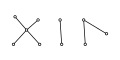
\includegraphics[width=0.4\textwidth]{gallois-part-2-star.pdf}
    \centering
  \end{figure}
  $G[C]$ consists of $k$ components: $|C| = |V(G)| - k$. A matching is obtained
  by chosing one edge from every star component of $G[C]$, the resulting matching
  has $k$ edges ($|M|$ = $k$)
  \begin{equation*}
    \alpha'(G) \geq |M| = k \geq |V(G)| -|C| = |V(G)| - \beta'(G)\\
  \end{equation*}
  \begin{equation*}
    \alpha'(G) + \beta'(G) \geq |V(G)|
  \end{equation*}
\end{itemize}
\end{proof}
\newpage
\section{Matchings}
Structure of the maximum matching $M$. For each $uv \in M$ one of these holds:
\begin{itemize}
\item[(1)] 
\begin{minipage}{.5\textwidth}
  \[
    N(u) \cap \overline{V(M)} = \emptyset
  \]
  \[
    N(v) \cap \overline{V(M)} = \emptyset
  \]
\end{minipage}% This must go next to `\end{minipage}`
\begin{minipage}{.5\textwidth}
  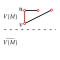
\includegraphics[width=0.45\textwidth]{max-matching-structure-1.pdf}
  \centering
\end{minipage}

\item[(2)] 
\begin{minipage}{.5\textwidth}
  \[
    N(u) \cap \overline{V(M)} \neq \emptyset
  \]
  \[
    N(v) \cap \overline{V(M)} \neq \emptyset
  \]
\end{minipage}% This must go next to `\end{minipage}`
\begin{minipage}{.5\textwidth}
  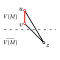
\includegraphics[width=0.45\textwidth]{max-matching-structure-2.pdf}
  \centering
\end{minipage}

\item[(3)]
\begin{minipage}{.20\textwidth}
  \[
    N(u) \cap \overline{V(M)} \neq \emptyset
  \]
  \[
    N(v) \cap \overline{V(M)} = \emptyset
  \]
\end{minipage}% This must go next to `\end{minipage}`
\begin{minipage}{.05\textwidth}
  or
  \centering
\end{minipage}% This must go next to `\end{minipage}`
\begin{minipage}{.20\textwidth}
  \[
    N(u) \cap \overline{V(M)} = \emptyset
  \]
  \[
    N(v) \cap \overline{V(M)} \neq \emptyset
  \]
\end{minipage}% This must go next to `\end{minipage}`
\begin{minipage}{.6\textwidth}
  \includegraphics[width=0.45\textwidth]{max-matching-structure-3.pdf}
  \centering
\end{minipage}
\end{itemize}
\begin{definition}
Let $M$ be a matching. A path $v_1u_1v_2u_2\dots v_k u_k (v_{k+1})$ is an \textbf{m-altering path} if the edges along
the path alternate between $M$ and $\overline{M} = E \ M$
\end{definition}
\begin{figure}[h]
  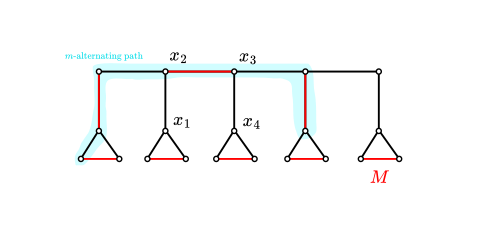
\includegraphics[width=0.8\textwidth]{m-alternating-example.pdf}
  \centering
\end{figure}
\begin{definition}
  An $m$-alternating path is $m$-augmenting if both ends of the path are uncovered by $M$
\end{definition}
For example $x_1x_2x_3x_4$ in the above figure.
This is important because $M'=M \setminus \{x_2x_3\}\cup \{x_1x_2\}$
is a larger matching.
\end{document}